\documentclass[12pt]{article} % Font size 12pt
\usepackage{fontspec}
\usepackage{polyglossia}
\usepackage{geometry}
\usepackage{algorithm}
\usepackage{algpseudocode}
\usepackage{hyperref} % For hyperlinks
\usepackage{amsmath}
\numberwithin{equation}{section}  % Reset equation counter with each section
\renewcommand{\theequation}{\arabic{section}-\arabic{equation}}
\usepackage{enumitem}

\usepackage{graphicx}      % For including images
\usepackage{caption}       % For customizing captions
\usepackage{subcaption}    % For subfigures within a figure

\usepackage{mathtools} % In preamble
\usepackage{amsfonts} % or \usepackage{amssymb}

\usepackage{comment}
\usepackage{ifthen}
\newboolean{showexamples}
\setboolean{showexamples}{true}  % or false to hide examples
% example boxes
\usepackage{tcolorbox}
\newtcolorbox{examplebox}[1]{%
  colback=white,
  colframe=gray!30,
  title={#1},
  sharp corners,
  boxrule=0.5pt,
  coltitle=black
}

\hypersetup{
    colorlinks=true,
    linkcolor=black,   % Internal links, those generated by cross-referenced elements
    filecolor=black,  % Links to local files
    urlcolor=black,    % Links to web sites
    citecolor=black,
}

\renewenvironment{examplebox}[1]{%
  \ifthenelse{\boolean{showexamples}}%
    {\begin{tcolorbox}[colback=white, colframe=gray!30, title={#1}, sharp corners, boxrule=0.5pt, coltitle=black]}%
    {\expandafter\comment}%
}{%
  \ifthenelse{\boolean{showexamples}}%
    {\end{tcolorbox}}%
    {\expandafter\endcomment}%
}

% Set fonts
\setmainfont{CMU Serif}
\newfontfamily\greekfont{CMU Serif}

% Define \greekfonttt
\newfontfamily\greekfonttt{DejaVu Sans Mono}[Script=Greek]

% Set languages
\setdefaultlanguage{greek}
\setotherlanguage{english}

% Set margins
\geometry{
    top=0cm,
    bottom=2cm,
    left=2cm,
    right=2cm
}

% modify the caption label for algorithms in the document to display "Αλγόριθμος" instead of Algorithm
\makeatletter
\renewcommand{\ALG@name}{Αλγόριθμος}
\makeatother

\setcounter{secnumdepth}{3} % Number subsubsections
\setcounter{tocdepth}{3}    % Show subsubsections in TOC

\title{\textbf{Προσομοίωση και Μοντελοποίηση \\ Δυναμικών Συστημάτων} \\ Τελική Εργασία}
\author{Αριστείδης Δασκαλόπουλος (ΑΕΜ: 10640)}
\date{\today}


\usepackage{titlesec}

% --- Sections ---
\titleformat{\section}
  {\normalfont\Large\bfseries} % Format: Large + bold
  {}                            % No label (number)
  {0pt}                         % Horizontal separation between label and title
  {}                            % Code before title
\titlespacing*{\section}        % Adjust spacing
  {0pt}                         % Left margin
  {3.5ex plus 1ex minus .2ex}   % Vertical space before
  {2.3ex plus .2ex}             % Vertical space after

% Format subsections as [X.Y] Title
\titleformat{\subsection}
  {\normalfont\large\bfseries}
  {[\thesubsection]} % Number in brackets
  {0.5em} % Space between number and title
  {}

% Format subsubsections as [X.Y.Z] Title  
\titleformat{\subsubsection}
  {\normalfont\normalsize\bfseries}
  {[\thesubsubsection]} % Number in brackets
  {0.5em} % Space between number and title
  {}

% Adjust spacing (optional)
\titlespacing*{\subsection}{0pt}{3.25ex plus 1ex minus .2ex}{1.5ex plus .2ex}
\titlespacing*{\subsubsection}{0pt}{3.25ex plus 1ex minus .2ex}{1.5ex plus .2ex}
  

\begin{document}
\maketitle


\renewcommand{\contentsname}{Περιεχόμενα}
\tableofcontents
\newpage
\newgeometry{
    top=2cm,
    bottom=2cm,
    left=2cm,
    right=2cm
}


\section{Θέμα 1}

% \vspace{-\topsep}
% \vspace{+2pt}
% \begin{center}
%     \textit{\textbf{Στόχος}: Εκτίμηση Άγνωστων Παραμέτρων με τις Μεθόδους Πραγματικού Χρόνου: \\Κλίσης και Lyapunov}
% \end{center}
% \vspace{-\topsep}
% \noindent\textrightarrow\ 

Το δοθέν γραμμικό σύστημα που καλούμαστε να μελετήσουμε είναι το εξής:

\vspace{-20pt}

\begin{align}\label{eq:sys_eq_1}
    \dot{x}(t) = A x(t) + B u(t),
\end{align}

\vspace{-\topsep}
% \vspace{+2pt}

\noindent όπου: 

\vspace{-\topsep}

\begin{center}
    $x(t) = \begin{bmatrix}x_1(t) & x_2(t)\end{bmatrix}^\top \in \mathbb{R}^2$ η κατάσταση του συστήματος, \hspace{0.5cm}
    $u(t) \in \mathbb{R}$ η είσοδος, \hspace{0.5cm} \\
    $A = \begin{pmatrix}
        a_{11} & a_{12} \\
        a_{21} & a_{22} \\
        \end{pmatrix}$ \hspace{0.25cm} και \hspace{0.25cm}
    $B = \begin{pmatrix}
        b_{1} \\
        b_{2} \\
        \end{pmatrix}$,
\end{center}

\vspace{-\topsep}

\noindent με τους $A$ και $B$ να θεωρούνται σταθεροί αλλά άγνωστοι/προς εκτίμηση πίνακες, 
για τα στοιχεία των οποίων γνωρίζουμε ότι ισχύουν οι παρακάτω περιορισμοί: 

\vspace{-\topsep}

\begin{center}
    \fbox{$a_{11} \in [-3, -1]$ \& $b_2 \in [1, +\infty)$}
\end{center}

% \vspace{+10pt}

Στα πλαίσια της ανάλυσής μας θεωρούνται μετρήσιμες οι καταστάσεις του συστήματος, $x_1(t)$ και $x_2(t)$, όπως και η είσοδος $u(t)$. 
Επίσης οι πραγματικές τιμές των παραμέτρων προς εκτίμηση είναι: 

\vspace{-\topsep}

\begin{table}[!ht]
    \centering
    \begin{tabular}{c c | c}
        \multicolumn{2}{c}{$A$} & $B$ \\
        $a_{11} = -2.15$ & $a_{12} = 0.25$ & $b_{1} = 0$ \\
        $a_{21} = -0.75$ & $a_{22} = -2$ & $b_{2} = 1.5$
    \end{tabular}
    % \caption{Caption}
    % \label{tab:my_label}
\end{table}

\vspace{-\topsep}
% \vspace{-10pt}

\noindent Μπορούμε εύκολα να δούμε ότι οι ιδιοτιμές του $2 \times 2$ πίνακα, $A$, είναι συζυγείς μιγαδικές και βρίσκονται στο ανοικτό αριστερό ημιεπίπεδο.

\begin{center}
    \textit{
    Στην συνέχεια θα παρουσιάσουμε έναν αλγόριθμο πραγματικού χρόνου (online) για την εκτίμηση των αγνώστων πινάκων, 
    θα μελετήσετε την ευστάθεια του συστήματος εκτίμησης που σχεδιάσαμε και, τέλος, θα εξάγουμε συμπεράσματα για την ακρίβεια των αποτελεσμάτων μας μέσω των ζητούμενων γραφικών παραστάσεων.
    }
\end{center}


\newpage

\newgeometry{
    top=2cm,
    bottom=2cm,
    left=2cm,
    right=2cm
}




\subsection{Ερώτημα Α}

Ο αλγόριθμος πραγματικού χρόνου για την εκτίμηση των $\hat{A}$ και $\hat{B}$ που θα παρουσιάσουμε στην παρακάτω ανάλυση εφαρμόζει την μέθοδο Lyapunov με προβολή\textemdash μιας και θέλουμε να κινούμαστε στον χώρο των λύσεων που ικανοποιούν τους περιορισμούς που αναφέραμε. Η δε δομή του συστήματος αναγνώρισης που επιλέγουμε να παρουσιάσουμε είναι η μεικτή (Μ) δομή (series-parallel configuration).

\subsubsection{Μαθηματική Ανάλυση Μεθόδου Lyapunov Μ δομής}

Στη Μ δομή, όπως γνωρίζουμε, χρησιμοποιούνται οι πραγματικές τιμές των \( x_1(t)\) και \( x_2(t) \) στο μοντέλο, οπότε έχουμε:
\begin{equation}\label{eq:estim_sys}
\dot{\hat{x}} = \hat{A}x + \hat{B}u + C(x - \hat{x}),
\end{equation}
όπου $\hat{A}$, $\hat{B}$: εκτιμήσεις των πινάκων $A$, $B$.

\vspace{+8pt}

\noindent\textbullet\hspace{0.2em} Το σφάλμα αναγνώρισης είναι $e = x - \hat{x}$ και παραγωγίζοντάς το ως προς τον χρόνο παίρνουμε:
\begin{equation}\label{eq:error_dot}
\dot{e} = A x + B u - \hat{A} x - \hat{B}u - Ce \xRightarrow{\substack{\tilde{A} = \hat{A} - A \\ \tilde{B} = \hat{B} - B}}
\dot{e} = - C e - \tilde{A} x - \tilde{B}u
\end{equation}


\noindent\textbullet\hspace{0.2em} Για την ανάλυσή μας ως συνάρτηση Lyapunov παίρνουμε την:
\begin{equation}\label{eq:lyapunov_b}
V = \frac{1}{2}e^{\top} e + \frac{1}{2}\text{tr}\{\tilde{A}^{\top}\tilde{A}\} + \frac{1}{2}\text{tr}\{\tilde{B}^{\top}\tilde{B}\}
\end{equation}
όπου με $\text{tr}\{\cdot\}$ συμβολίζουμε το ίχνος (trace) ενός πίνακα. Αν παραγωγίσουμε την $V$ ως προς τον χρόνο κατά μήκος της λύσης της \eqref{eq:error_dot} βρίσκουμε:
\begin{equation}\label{eq:vdot_initial_b}
\dot{V} = e^{\top} \dot{e} + \text{tr}\{\tilde{A}^{\top}\dot{\hat{A}}\} + \text{tr}\{\tilde{B}^{\top}\dot{\hat{B}}\} \overset{\eqref{eq:error_dot}}{=}
- e^{\top} C e - e^{\top} \tilde{A} x - e^{\top} \tilde{B}u + \text{tr}\{\tilde{A}^{\top}\dot{\hat{A}}\} + \text{tr}\{\tilde{B}^{\top}\dot{\hat{B}}\}.
\end{equation}
Επίσης γνωρίζουμε από τις ιδιότητες του trace ότι:
\begin{equation*}
e^{\top} \tilde{A} x = \text{tr}\{\tilde{A} x e^{\top}\} \quad\& \quad
\text{tr}\{\tilde{A}^{\top}\dot{\hat{A}}\} = \text{tr}\{\tilde{A}\dot{\hat{A}}^{\top}\}
\quad \text{(ομοίως για $B$)}
\end{equation*}
και έτσι η \eqref{eq:vdot_initial_b} γράφεται:
\begin{equation}\label{eq:vdot_intermediate_b}
\dot{V} = - e^{\top} C e + \text{tr}\{\tilde{A}\dot{\hat{A}}^{\top} + \tilde{B}\dot{\hat{B}}^{\top} - \tilde{A} x e^{\top} - \tilde{B}u e^{\top}\}.
\end{equation}



\vspace{+8pt}

\noindent\textbullet\hspace{0.2em} Για να απαλειφθούν οι όροι των οποίων το πρόσημο δεν γνωρίζουμε στην παράγωγο της Lyapunov, επιλέγουμε:
\begin{equation}\label{eq:adapt_A_B}
\dot{\hat{A}}^{\top} = x e^{\top} \quad \& \quad
\dot{\hat{B}}^{\top} = u e^{\top} \quad \Rightarrow \quad
\dot{\hat{A}} = e x^{\top} \quad \& \quad
\dot{\hat{B}} = e u^{\top},
\end{equation}
και τότε η \eqref{eq:vdot_intermediate_b} γίνεται:
\begin{equation}\label{eq:vdot_final_b}
\dot{V} = - e^{\top} C e \leq 0, \ \text{όπου ο πίνακας $C$ πρέπει να είναι θετικά (ημι)ορισμένος.}
\end{equation}

\begin{examplebox}{}
    Άρα ο αλγόριθμος με προβολή που θα αναπτύξουμε στην συνέχεια θα ακολουθεί την λύση \eqref{eq:adapt_A_B} που παρέχει η παραπάνω μέθοδος 
    (με εξαίρεση τις περιπτώσεις που φτάνουμε στο σύνορο, όπως θα εξηγήσουμε).
    Με το παραπάνω βλέπουμε επίσης πως με κατάλληλη επιλογή του πίνακα $C$ η μέθοδος (χωρίς προβολή) είναι ευσταθής. 
    (Για την σύγκληση των παραμετρικών σφαλμάτων στο μηδέν πρέπει επίσης η είσοδος να ικανοποιεί μια ΣΕΔ).
\end{examplebox}

\vspace{+5pt}



\subsubsection{Αλγόριθμος Lyapunov με Προβολή}

Για την ανάπτυξη του αλγορίθμου με προβολή ορίζουμε:
\begin{equation}\label{eq:theta_vect}
\theta = \begin{bmatrix} a_{11} & a_{12} & a_{21} & a_{22} & b_{1} & b_{2} \end{bmatrix}^\top \in \mathbb{R}^6,
\end{equation}
συνεπώς λαμβάνοντας υπόψιν την \eqref{eq:adapt_A_B} θα έχουμε (για την περίπτωση χωρίς περιορισμούς):
\begin{equation}\label{eq:theta_dot}
    \dot{\hat{\theta}} = 
    \begin{bmatrix} 
    \dot{\hat{a}}_{11} & \dot{\hat{a}}_{12} & \dot{\hat{a}}_{21} & \dot{\hat{a}}_{22} & \dot{\hat{b}}_{1} & \dot{\hat{b}}_{2} 
    \end{bmatrix}^\top 
    \overset{\eqref{eq:adapt_A_B}}{=} 
    \begin{bmatrix} 
    e_1 x_1 & e_1 x_2 & e_2 x_1 & e_2 x_2 & e_1 u & e_2 u
    \end{bmatrix}^\top, 
\end{equation}
η οποία σχέση προέκυψε αντικαθιστώντας στην \eqref{eq:adapt_A_B} τα $x = \begin{bmatrix}x_1 & x_2\end{bmatrix}^\top$ και $e = \begin{bmatrix}e_1 & e_2\end{bmatrix}^\top$.

\vspace{+5pt}

Ορίζουμε τώρα το κυρτό σύνολο $\Theta$ όλων των $\hat{\theta}$ που να ικανοποιούν τους περιορισμούς:
\begin{equation}\label{eq:Theta_def}
\Theta = \{ \hat{\theta} \in \mathbb{R}^6 : g_1(\hat{\theta}) \le 0, g_2(\hat{\theta}) \le 0, g_3(\hat{\theta}) \le 0 \},
\end{equation}
όπου τα $g_i(\hat{\theta})$, για $i  = 1, 2, 3$, ορίζονται παρακάτω έτσι, ώστε οι ανισότητες στη \eqref{eq:Theta_def} να εκφράζουν τους αρχικούς μας περιορισμούς:
\begin{center}
    $g_1(\hat{\theta}) = - \hat{a}_{11} - 3$, \hspace{0.5cm}
    $g_2(\hat{\theta}) = \hat{a}_{11} + 1$, \hspace{0.5cm}
    $g_3(\hat{\theta}) = - \hat{b}_{2} + 1$. 
\end{center}

\begin{examplebox}{Σχόλιο}
    Ο διανυσματικός ορισμός του $g(\hat{\theta})$ μπορεί να διατυπωθεί ως:
    $$
    g(\hat{\theta}) = \begin{bmatrix}
        g_1 & g_2 & g_3
    \end{bmatrix}^\top \in \mathbb{R}^3.
    $$
    Τότε στην έκφραση των περιορισμών στην \eqref{eq:Theta_def} θα είχαμε την διανυσματική ανισότητα: $g(\hat{\theta}) < 0_{3 \times 1}$. 
    Αυτή η μορφή είναι μαθηματικά ισοδύναμη με την ανάλυση καθενός από τους επιμέρους όρους/συνιστώσες $g_i < 0$, για $i = 1, 2, 3$. 
\end{examplebox}

\vspace{+5pt}

Για την ανάπτυξη του αλγορίθμου με προβολή, εκκινούμε από ένα αρχικό σημείο $\hat{\theta}(0) = \hat{\theta}_0$ το οποίο βρίσκεται στο εσωτερικό του συνόλου $\Theta$, και ακολουθούμε τη δυναμική που υπαγορεύεται από τη Σχέση~\eqref{eq:theta_dot} (που δεν λαμβάνει υπόψιν τους περιορισμούς). 
Όταν η τροχιά φτάσει στο σύνορο του $\Theta$\textemdash δηλαδή όταν για κάποιο $i \in {1, 2, 3}$ ισχύει $g_i(\hat{\theta}) = 0$\textemdash εξετάζεται αν το $\hat{\theta}$ τείνει να κινηθεί εκτός του επιτρεπτού συνόλου $\Theta$, και έχουμε περιπτώσεις:
\begin{itemize}[noitemsep, nolistsep]
    \item Εάν αυτό δεν συμβαίνει, συνεχίζουμε να εφαρμόζουμε την ίδια δυναμική. 
    \item Σε αντίθετη περίπτωση, \textit{\textbf{προστίθεται κατάλληλος όρος}}, ο οποίος εξαναγκάζει την κίνηση του $\hat{\theta}$ προς το εσωτερικό του $\Theta$ ή κατά μήκος του συνόρου του.
\end{itemize}

Σύμφωνα με τα παραπάνω προκύπτει ο αλγόριθμος με προβολή ως:
\begin{equation}\label{eq:theta_dot_proj}
\dot{\hat{\theta}} = 
\begin{cases} 
    \Gamma \begin{bmatrix} e_1 x_1 \\ e_1 x_2 \\ e_2 x_1 \\ e_2 x_2 \\ e_1 u \\ e_2 u \end{bmatrix}, 
    & \begin{split}
        \text{αν } \hat{\theta} \in \Theta_{in} \text{ \textit{ή αν} } \\
        \hat{\theta} \in \Theta_b \quad  \& \quad \dot{\hat{\theta}}^{\top}_{\eqref{eq:theta_dot}} \cdot \nabla g \le 0_{3 \times 1}
    \end{split} \\
    \Gamma \begin{bmatrix} e_1 x_1 \\ e_1 x_2 \\ e_2 x_1 \\ e_2 x_2 \\ e_1 u \\ e_2 u \end{bmatrix} - \Gamma \frac{\nabla g \nabla g^{\top}}{\nabla g^{\top} \Gamma \nabla g} \Gamma \begin{bmatrix} e_1 x_1 \\ e_1 x_2 \\ e_2 x_1 \\ e_2 x_2 \\ e_1 u \\ e_2 u \end{bmatrix}, & \text{διαφορετικά}
\end{cases}
\end{equation}
όπου \(\Theta_{in}\) είναι το εσωτερικό και \(\Theta_b\) το σύνορο του $\Theta$. Στην \eqref{eq:theta_dot_proj} πρέπει \(\hat{\theta}(0) \in \Theta\). 

Για την \eqref{eq:theta_dot_proj} ισχύουν τα εξής:
\begin{itemize}[noitemsep, nolistsep]
    \item Ο πίνακας $\Gamma = \begin{bmatrix}
        \gamma_1 & 0        & \cdots & 0 \\
        0        & \gamma_2 & \cdots & 0 \\
        \vdots    & \vdots   & \ddots & \vdots \\
        0        & 0        & \cdots & \gamma_6
    \end{bmatrix} \in \mathbb{R}^{6 \times 6}$
    περιλαμβάνει όλες τις μεταβλητές $\gamma_i > 0$ (learning rate) με τις οποίες θα πολλαπλασιαστεί καθεμία συνιστώσα του διανύσματος $\dot{\hat{\theta}}$.

    \item Όταν το $g$ εκφράζει διανυσματικά όλους τους περιορισμούς ισχύει: 
        $$\nabla g = \begin{bmatrix}
            \nabla g_1 & \nabla g_2 & \nabla g_3
        \end{bmatrix}\in \mathbb{R}^{6 \times 3},$$
        όπου: 
        \begin{equation}\label{eq:grad_g}
            \nabla g_1 = \begin{bmatrix}
                -1 & 0 & 0 & 0 & 0 & 0
            \end{bmatrix}^{\top}, \quad 
            \nabla g_2 = \begin{bmatrix}
                1 & 0 & 0 & 0 & 0 & 0
            \end{bmatrix}^{\top}, \quad 
            \nabla g_3 = \begin{bmatrix}
                0 & 0 & 0 & 0 & 0 & -1
            \end{bmatrix}^{\top}
        \end{equation}

        \item Ο λόγος $\frac{\nabla g \nabla g^\top}{\nabla g^\top \Gamma \nabla g} \in \mathbb{R}^{6 \times 6}$ εκφράζει τον μηχανισμό με τον οποίο προβάλλεται το διάνυσμα $\hat{\theta}$ εντός του επιτρεπτού χώρου $\Theta$, όταν διαπιστώνεται ότι τείνει να κινηθεί εκτός αυτού\textemdash δηλαδή, όταν ο πρώτος κλάδος είτε οδηγεί σε τιμή εκτός του $\Theta$, είτε δίνει σημείο στο σύνορό του, αλλά με παράγωγο $\dot{\hat{\theta}}$ που έχει φορά προς το εξωτερικό του συνόλου.

        Για τον δε υπολογισμό του λόγου αυτού η μαθηματική ισοδυναμία ώστε να οδηγεί σε προβολή στο $\Theta$ είναι:  $\nabla g (\nabla g^\top \Gamma \nabla g)^{-1} \nabla g^\top$.

        \begin{examplebox}{Παρατήρηση}
            Για οποιοδήποτε διαγώνιο πίνακα $\Gamma$ κατόπιν αντικατάστασης και εύρεσης του $\nabla g^\top \Gamma \nabla g$, παρατηρούμε ότι αυτός είναι ιδιάζον (μη αντιστρέψιμος/με ορίζουσα μηδέν). 
            Αυτό συμβαίνει επειδή οι περιορισμοί που εκφράζουν οι συναρτήσεις $g_1$ και $g_2$ αναφέρονται στην ίδια παράμετρο $a_{11}$ και δεν γίνεται και οι δύο ταυτόχρονα να είναι $\ge 0$.
            Άρα η έκφραση του λόγου ως αντίστροφος πίνακας, όπως δείξαμε προηγουμένως, δεν μπορεί να εφαρμοστεί στην περίπτωσή μας. 
        \end{examplebox} 
        
\end{itemize}


Για την επίλυση του προβλήματος, στην περίπτωση όπου πρέπει να πάρουμε τον δεύτερο κλάδο της \eqref{eq:theta_dot_proj}, θα προβάλουμε την λύση λαμβάνοντας μόνο τους ενεργούς περιορισμούς. Ένας τρόπος να το κάνουμε αυτό είναι ο παρακάτω:

Τροποποιούμε τον αλγόριθμο που παρουσιάζει η \eqref{eq:theta_dot_proj}\textemdash και συγκεκριμένα τον δεύτερο κλάδο που κάνει την προβολή\textemdash ώστε να χρησιμοποιούμε άθροισμα επί των περιορισμών.
Επομένως, στον τροποποιημένο αλγόριθμο, ο όρος προβολής ανανεώνεται ως:

\begin{equation}\label{t1:theta_update}
    \dot{\hat{\theta}} = 
    \Gamma \begin{bmatrix} e_1 x_1 \\ e_1 x_2 \\ e_2 x_1 \\ e_2 x_2 \\ e_1 u \\ e_2 u \end{bmatrix} - 
    \sum_{i \in \mathcal{A}} \Gamma \frac{\nabla g_i \nabla g_i^{\top}}{\nabla g_i^{\top} \Gamma \nabla g_i} \Gamma \begin{bmatrix} e_1 x_1 \\ e_1 x_2 \\ e_2 x_1 \\ e_2 x_2 \\ e_1 u \\ e_2 u \end{bmatrix},
\end{equation}

ή για απλότητα:

\begin{equation}\label{eq:update_theta}
    \dot{\hat{\theta}}_{new} = 
    \Gamma \dot{\hat{\theta}}_{current} - 
    \sum_{i \in \mathcal{A}} \Gamma \frac{\nabla g_i \nabla g_i^{\top}}{\nabla g_i^{\top} \Gamma \nabla g_i} \Gamma \dot{\hat{\theta}}_{current},
\end{equation}

όπου \(\mathcal{A}\) είναι το σύνολο των \textit{ενεργών περιορισμών}\textemdash δηλαδή, οι δείκτες \(i\) για τους οποίους είτε \(g_i(\hat{\theta}) > 0\), είτε \(g_i(\hat{\theta}) = 0 \ \& \ \dot{\hat{\theta}}_{\eqref{eq:theta_dot}} \cdot \nabla g_i > 0\). 

\begin{examplebox}{}
    Με \(\dot{\hat{\theta}}_{\eqref{eq:theta_dot}}\) συμβολίζουμε την \textit{χωρίς περιορισμούς} επόμενη ενημέρωση του διανύσματος $\dot{\hat{\theta}}_{current}$ (ακολουθώντας την μέθοδο Lyapunov για την Μ δομή). 
\end{examplebox}


Το άθροισμα επί των ενεργών περιορισμών εμφανίζεται επειδή, όταν πολλαπλοί περιορισμοί είναι ενεργοί (παρατηρώντας τους περιορισμούς μπορούμε να έχουμε max δύο ενεργούς περιορισμούς: $g_1$ με $g_3$ ή $g_2$ με $g_3$), η ενημέρωση πρέπει να προβληθεί ως προς όλους τους ενεργούς περιορισμούς.

Ο όρος $\Gamma \frac{\nabla g_i \nabla g_i^{\top}}{\nabla g_i^{\top} \Gamma \nabla g_i} \Gamma \dot{\hat{\theta}}$ προβάλλει την ενημέρωση \(\dot{\hat{\theta}}\) στην κάθετη κατεύθυνση της \(i\)-οστής επιφάνειας περιορισμού, $g_i(\hat{\theta}) = 0$. 
Η αφαίρεση του αποτελέσματος της προβολής αφαιρεί τη συνιστώσα του \(\dot{\hat{\theta}}\) που θα παραβίαζε το \( g_i(\hat{\theta}) \leq 0 \). 
Όταν πολλαπλοί περιορισμοί είναι ενεργοί, αθροίζουμε αυτές τις προβολές για να αφαιρέσουμε τις συνιστώσες κατά μήκος όλων των σχετικών κάθετων κατευθύνσεων,
διασφαλίζοντας ότι η ενημέρωση του \(\dot{\hat{\theta}}\) παραμένει στο σύνορο $\Theta_b$.

Ο λόγος για τον οποίο το άθροισμα στην \eqref{eq:update_theta} είναι μαθηματικά σωστό είναι επειδή σε περίπτωση που έχουμε πολλαπλούς ενεργούς περιορισμούς, τότε όπως εξηγήσαμε αυτό σημαίνει ότι $\mathcal{A} = \{1, 3\} \ \text{ή} \ \{2, 3\}$.
Άρα, επειδή από τις \eqref{eq:grad_g} έχουμε $\nabla g_1^{\top} \cdot \nabla g_3 = 0$ και $\nabla g_2^{\top} \cdot \nabla g_3 = 0$, 
επομένως οι προβολές ως προς αυτά τα ζεύγη είναι μεταξύ τους ορθογώνιες και έπεται πως μπορούν να υπολογιστούν και να αφαιρεθούν ανεξάρτητα οι συνιστώσες που δίνουν. 
Εναλλακτικά, θα έπρεπε να σχηματίζουμε κάθε φορά ένα διάνυσμα $g'$ με όλους τους ενεργούς περιορισμούς.




\vspace{+10pt}

\begin{center}
    \textit{Έχοντας πλέον ολοκληρώσει την θεωρητική ανάλυση του προβλήματος μπορούμε να συνεχίσουμε με την συνοπτική ανάλυση του τρόπου προσομοίωσης/επίλυσης του προβλήματος στο MATLAB.}
\end{center}

\newpage

\subsubsection{Προσομοίωση στο MATLAB}

Συνοψίζοντας την ανάλυση της προηγούμενης ενότητας, για την εύρεση των προς εκτίμηση παραμέτρων, έχουμε καταλήξει στο εξής σύστημα προς επίλυση:

\noindent\textbullet\hspace{0.2em} Η πρώτη διαφορική εξίσωση που θέλουμε να λύσουμε είναι αυτή του πραγματικού συστήματος, 
καθώς για κάθε χρονική στιγμή πρέπει να γνωρίζουμε την $x(t)$ (η μέθοδος είναι πραγματικού χρόνου επομένως λύνουμε με \textit{ode45} αυτήν την διαφορική, ταυτόχρονα με όλες τις υπόλοιπες):
\begin{equation}
    \dot{x}(t) = A_{\text{true}} x(t) + B_{\text{true}} u(t),
\end{equation}
όπου \( x(t) \in \mathbb{R}^2 \) είναι το διάνυσμα κατάστασης και \( u(t) \in \mathbb{R} \) είναι ένα γνωστό σήμα εισόδου της επιλογής μας (θα αναφερθούμε στην επιλογή του παρακάτω).  

\noindent\textbullet\hspace{0.2em} Η δεύτερη διαφορική αναφέρεται στο σύστημα αναγνώρισης. Οι πίνακες \( A_{\text{true}} = A \in \mathbb{R}^{2 \times 2} \) και \( B_{\text{true}} = B \in \mathbb{R}^{2 \times 1} \) για το πάνω σύστημα θεωρούνται γνωστοί, 
όμως θα πρέπει να εκτιμηθούν από το σύστημα αναγνώρισης το οποίο ορίστηκε στην προηγούμενη ανάλυση με την παρακάτω μεικτή δομή:
\begin{equation}
    \dot{\hat{x}}(t) = A_{\text{hat}} x(t) + B_{\text{hat}} u(t) + C \left( x(t) - \hat{x}(t) \right),
\end{equation}
όπου:
\[
\hat{A} = A_{\text{hat}} = 
\begin{bmatrix}
\hat\theta_1 & \hat\theta_2 \\
\hat\theta_3 & \hat\theta_4
\end{bmatrix}, \quad
\hat{B} = B_{\text{hat}} = 
\begin{bmatrix}
\hat\theta_5 \\
\hat\theta_6
\end{bmatrix}, \quad
e(t) = x(t) - \hat{x}(t), \quad 
C = \theta_{m} \cdot I_2,
\]
με το $\theta_{m}$ να πρέπει να είναι θετικός αριθμός της επιλογής μας, ώστε να ικανοποιείται η \eqref{eq:vdot_final_b}.

\noindent\textbullet\hspace{0.2em} Τέλος το σύστημά μας πρέπει να περιλαμβάνει τον νόμο ενημέρωσης παραμέτρων (με περιορισμούς).
Ο αντίστοιχος νόμος χωρίς περιορισμούς δίνεται από την \eqref{eq:theta_dot}, 
και κλιμακώνεται από έναν θετικά ορισμένο διαγώνιο πίνακα \( \Gamma = \mathrm{diag}(\gamma_1, \ldots, \gamma_6) \).
Για την δε επιβολή περιορισμών στις παραμέτρους, εφαρμόζεται η μέθοδος προβολής της \eqref{eq:update_theta}.


Άρα, το πλήρες σύστημα που θα δώσουμε στην \textit{ode45} για επίλυση είναι το εξής:
\begin{equation}
\frac{d}{dt}
\begin{bmatrix}
x(t) \\
\hat{x}(t) \\
\theta(t)
\end{bmatrix}
=
\begin{bmatrix}
A_{\text{true}} x(t) + B_{\text{true}} u(t) \\
A_{\text{hat}} x(t) + B_{\text{hat}} u(t) + C (x(t) - \hat{x}(t)) \\
\text{Proj}\left( \hat\theta_{\text{current}}, \Gamma \dot{\hat\theta}_{\text{current}} \right)
\end{bmatrix},
\end{equation}
με κατάλληλες αρχικές τιμές για τα $x_0$, $\hat{x}_0$ και $\hat\theta_0$.

\begin{examplebox}{Σχόλιο}
    Η συνάρτηση προβολής $\text{Proj}\left( \hat\theta_{\text{current}}, \Gamma \dot{\hat\theta}_{\text{current}}  \right)$ 
    παίρνει ως όρισμα και το $\hat\theta_{\text{current}}$ για να ελέγξει το εσωτερικό γενόμενο αυτού με τις παραγώγους των συναρτήσεων περιορισμών, 
    \eqref{eq:grad_g}\textemdash μιας και με βάση το πρόσημο του αποτελέσματος βρίσκει αν και ποιοι εκ των περιορισμών είναι ενεργοί ώστε να κάνει την αντίστοιχη προβολή. 
\end{examplebox}

Στο αρχείο \textit{src/constrainedSystemDynamics.m} έχει εκφραστεί το παραπάνω σύστημα, 
το οποίο λύνεται (με \textit{ode45}) στο εκτελέσιμο script: \underline{\textit{mainPart1a.m}} που αντιστοιχεί στο Ερώτημα α του Θέματος 1.


\subsubsection{Μελέτη Ευστάθειας Συστήματος Εκτίμησης \& Επιλογή Εισόδου $u(t)$}

Στην μαθηματική ανάλυση της μεθόδου Lyapunov για μεικτή δομή συστήματος αναγνώρισης δείξαμε ότι το σύστημα εκτίμησης είναι ευσταθές αν ο πίνακας $C$
της \eqref{eq:vdot_intermediate_b} είναι θετικά ημιορισμένος. 
Παρόλα αυτά η παραπάνω ανάλυση αφορούσε την περίπτωση που έχουμε ενημέρωση των παραμέτρων $\theta$, χωρίς περιορισμούς, μέσω της \eqref{eq:theta_dot}.
Για την περίπτωση που η δυναμική του $\theta$ δίνεται από την \eqref{eq:update_theta}, γεννιέται το ερώτημα αν αυτό θα επηρεάσει την ευστάθεια του συστήματος εκτίμησης. 
Παρόλα αυτά, με την προβολή του $\theta$ σύνορο\textemdash 
φράσσοντας δηλαδή το επιτρεπτό πεδίο στο οποίο μπορούν να κινηθούν τα $\hat\theta$\textemdash 
όχι απλώς δεν "χαλάει" η συνθήκη ευστάθειας της \eqref{eq:vdot_intermediate_b}, αλλά στην πράξη γίνεται ακόμα πιο αρνητική.

Πράγματι, αντικαθιστώντας την \eqref{t1:theta_update} στην \eqref{eq:vdot_intermediate_b}, παρατηρούμε ότι μέσα στο trace θα μείνουν μόνο τα στοιχειά, που αναφέρονται στην προβολή. 
Με αυτά, το αποτέλεσμα του trace δίνει μία αρνητική ποσότητα η οποία δεν επηρεάζει την συνθήκη $\dot{V} < 0$.
Προφανώς η επιλογή κατάλληλου πίνακα $C$ είναι σε κάθε περίπτωση σημαντική για την ευστάθεια.

Ένας τρόπος που μπορούμε να επαληθεύσουμε και στην πράξη την ευστάθεια του συστήματος εκτίμησης 
είναι να δοκιμάσουμε να τρέξουμε την προσομοίωση με διάφορες εισόδους $u(t)$ και να δούμε ότι όντως στο σύστημά μας υπάρχει ευστάθεια.
Η επιλογή κατάλληλης εισόδου είναι επίσης σημαντική μιας και από αυτήν (όπως αναφέραμε και στο τέλος της μαθηματική ανάλυση της μεθόδου Lyapunov)
θα εξαρτηθεί αν τα παραμετρικά σφάλματα θα συγκλίνουν στο μηδέν με την πάροδο του χρόνου.  

Ικανή και αναγκαία συνθήκη για να συγκλίνει η εκτίμηση των παραμέτρων $\hat\theta$ στην πραγματική τους τιμή $\theta$ είναι η ικανοποίηση μιας ΣΕΔ.
Εφόσον μας δίνεται η δυνατότητα η $u(t)$ να είναι δικής μας επιλογής, επιλέγουμε την:
\begin{equation}\label{t1:u}
    u(t) = 2.5  \sin(t) + 1.5  \cos(1.5 t) + 0.8  \sin(3 t).
\end{equation}
Στην πράξη, για το ΓΧΑ σύστημα 2ης τάξης που μελετάμε, μας ενδιαφέρει να εκτιμήσουμε και τις $6$ \textit{ανεξάρτητες} παραμέτρους του.
Γι' αυτόν τον λόγο, επιλέγουμε να χρησιμοποιήσουμε συνολικά τρεις συχνότητες.
Με αυτόν τον τρόπο εξασφαλίζουμε ότι το σήμα εισόδου έχει αρκετές συχνότητες ώστε να έχουμε την δυνατότητα να εκτιμήσουμε με αρκετή ακρίβεια καθεμία από τις $6$ παραμέτρους του (με σφάλμα εκτίμηση κάθε παραμέτρου να μπορεί ιδανικά να τείνει στο μηδέν). 


\begin{center}
    \textit{Στην συνέχεια παραθέτουμε τις ζητούμενες γραφικές παραστάσεις και εξάγουμε σχετικά συμπεράσματα.}
\end{center}



\subsubsection{Αποτελέσματα MATLAB και Συμπεράσματα}

Στο Σχήμα~\ref{fig:x_est} παρουσιάζονται οι γραφικές παραστάσεις των δύο καταστάσεων $x(t) = [x_1(t) \ \ x_2(t)]^{\top}$.
Όπως είναι φανερό και οπτικά, αλλά και όπως δείχνουν οι αντίστοιχες γραφικές παραστάσεις των σφαλμάτων στο Σχήμα~\ref{fig:err}, 
το σφάλμα της μοντελοποίησης τείνει στο μηδέν με την πάροδο του χρόνου\textemdash 
όπως ακριβώς περιμέναμε να συμβαίνει και σύμφωνα με την θεωρητική ανάλυση. 

Στο αρχείο \textit{mainTopic1a.m} μπορούμε να αλλάξουμε τον συνολικό χρόνο προσομοίωσης μέσω της μεταβλητής {\small \texttt{T\_final}},
όπως επίσης και τις τιμές των $\theta_m$ και $\Gamma$ μέσω των {\small\texttt{c\_coeff}} και {\small \texttt{gamma}} αντίστοιχα. 
Μπορούμε επίσης να αλλάξουμε τις αρχικές τιμές/σημείο εκκίνησης, προσέχοντας όμως η αρχική τιμή $\theta_0$ να ανήκει στο $\Theta$.

Στο Σχήμα~\ref{fig:A_est} βλέπουμε τις γραφικές παραστάσεις των $[A]_{ij}$ ως προς τον χρόνο. 
Όπως είναι φανερό, με το πέρας του χρόνου, καθεμία από αυτές τείνει να συγκλίνει προς την πραγματική της τιμή.
Αξίζει να επισημάνουμε ότι στην περίπτωση της γραφικής παράστασης του $a_{11}$, αρχικά η λύση πάει να βγει εκτός επιτρεπτών τιμών 
αλλά παρόλα αυτά προβάλλεται στο σύνορο $\Theta_b$, όπως ακριβώς αναλύσαμε στην θεωρία ότι θα συνέβαινε. 

Τέλος το Σχήμα~\ref{fig:B_est} περιέχει τις προβλέψεις που αφορούν τις παραμέτρους $[B]_{i}$ με τον χρόνο. 
Και σε αυτήν την περίπτωση, όπως και με τις προηγούμενες, βλέπουμε ότι όσο περνάει ο χρόνος οι τιμές των παραμέτρων προσαρμόζονται κατάλληλα και τείνουν σε αυτές του πραγματικού συστήματος. 
Αυτό περιμέναμε να το δούμε, μιας και η μέθοδος που έχουμε εφαρμόσει είναι πραγματικού χρόνου.

Τέλος παραθέτουμε τα logs που τυπώνουμε, τα οποία αναφέρονται στο σχετικό σφάλμα της τελικής εκτίμησης σε σχέση με την πραγματική τιμή για την κάθε παράμετρο. 
Με χρήση διαφορετικής εισόδου ή με την αλλαγή των $\Gamma$ και $\theta_m$, μπορούμε να πετύχουμε διαφορετικά tradeoff μεταξύ των προβλέψεων των παραμέτρων.
\begin{figure}[ht!]
    \centering
    \begin{minipage}{0.48\textwidth}
        \centering
        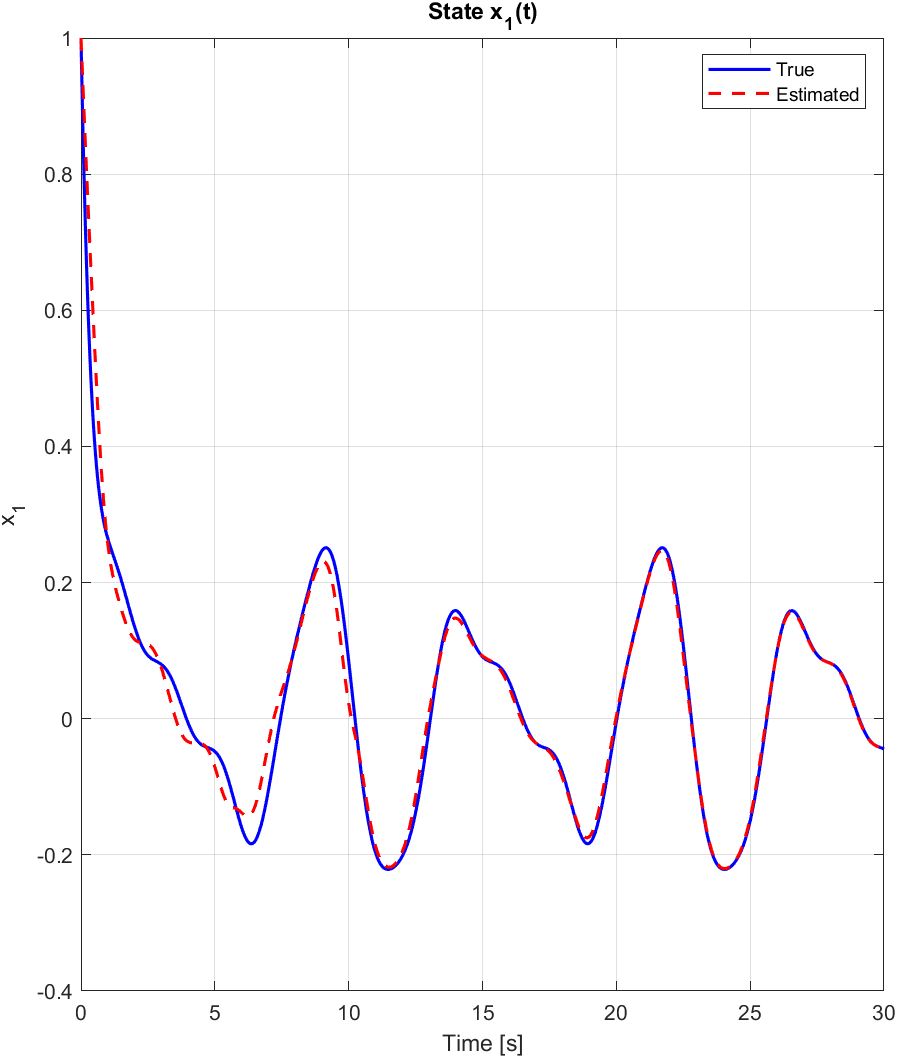
\includegraphics[width=0.8\linewidth]{plots/plot1_a_x1.png}
        % \caption{Image 1}
    \end{minipage}
    \hfill
    \begin{minipage}{0.48\textwidth}
        \centering
        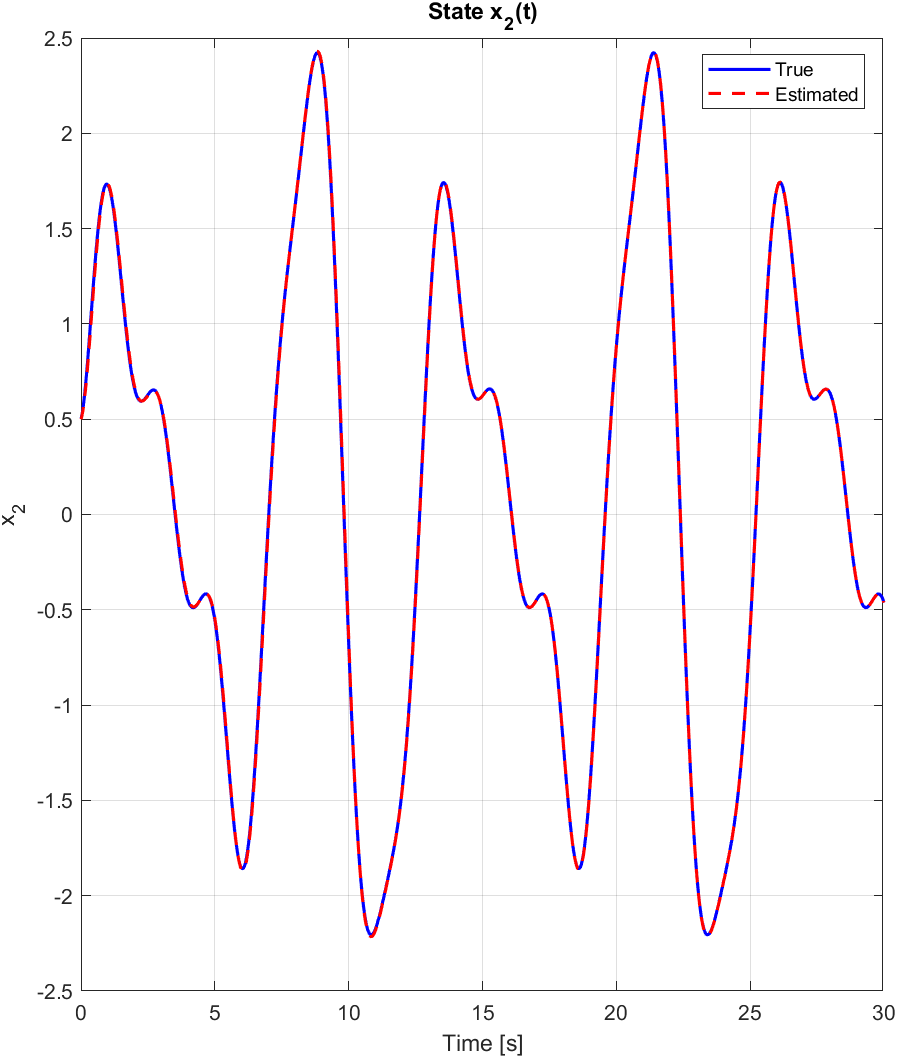
\includegraphics[width=0.8\linewidth]{plots/plot1_b_x2.png}
        % \caption{Image 2}
    \end{minipage}
    
    \caption{}
    \label{fig:x_est}
\end{figure}

\begin{figure}[ht!]
    \centering
    \begin{minipage}{0.32\textwidth}
        \centering
        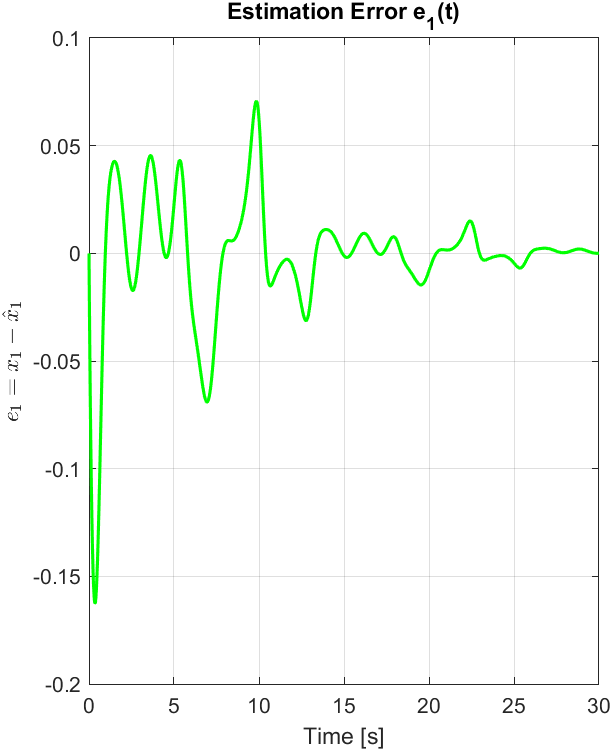
\includegraphics[width=0.99\linewidth]{plots/plot2_a_e1.png}
        % \caption{Image 1}
    \end{minipage}
    \hfill
    \begin{minipage}{0.32\textwidth}
        \centering
        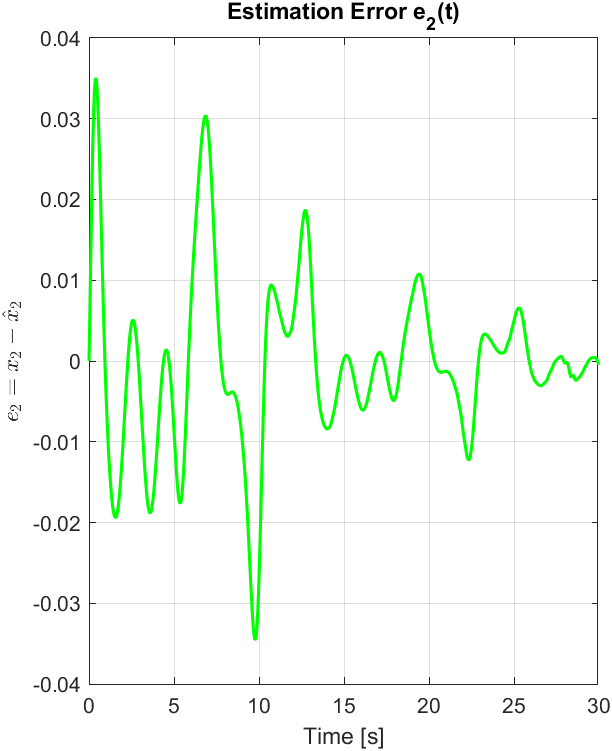
\includegraphics[width=0.99\linewidth]{plots/plot2_b_e2.png}
        % \caption{Image 2}
    \end{minipage}
    \hfill
    \begin{minipage}{0.32\textwidth}
        \centering
        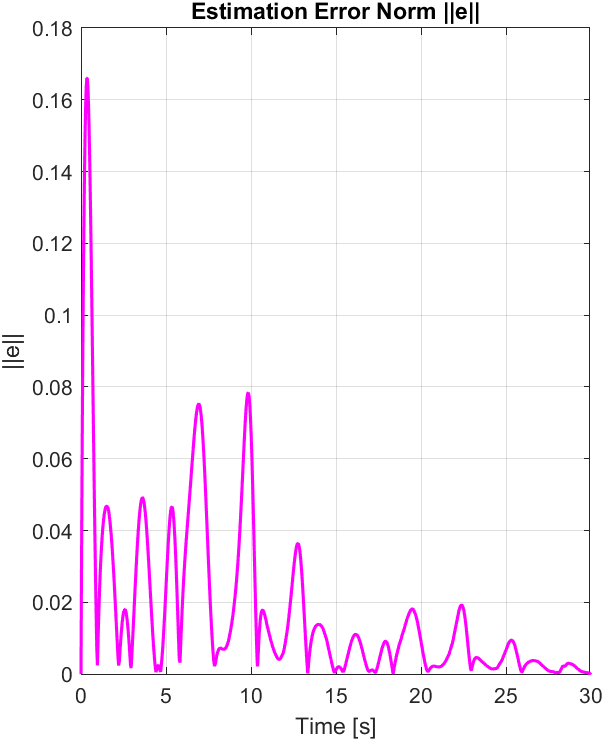
\includegraphics[width=0.99\linewidth]{plots/plot2_c_eNorm.png}
        % \caption{Image 2}
    \end{minipage}
    
    \caption{}
    \label{fig:err}
\end{figure}

\begin{figure}[ht!]
    \centering
    \begin{minipage}{0.48\textwidth}
        \centering
        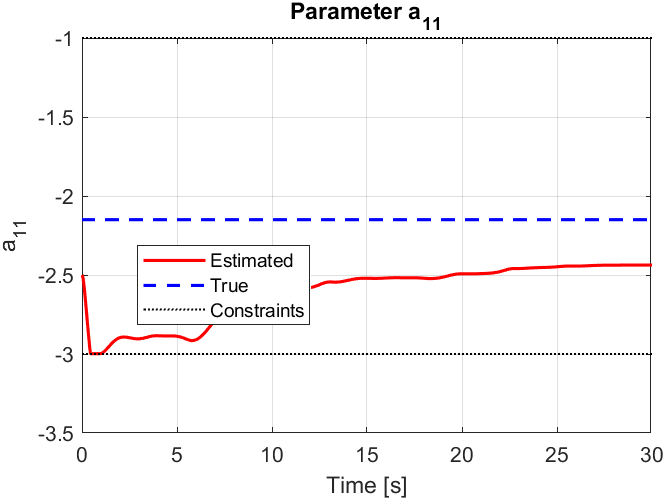
\includegraphics[width=0.8\linewidth]{plots/plot3_a_a11.png}
        % \caption{Image 1}
    \end{minipage}
    \hfill
    \begin{minipage}{0.48\textwidth}
        \centering
        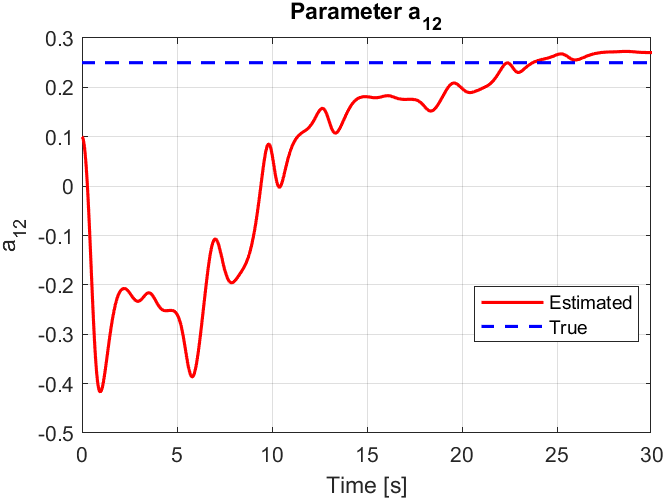
\includegraphics[width=0.8\linewidth]{plots/plot3_b_a12.png}
        % \caption{Image 2}
    \end{minipage}
    
    \vspace{1em} % Space between rows
    
    \centering
    \begin{minipage}{0.48\textwidth}
        \centering
        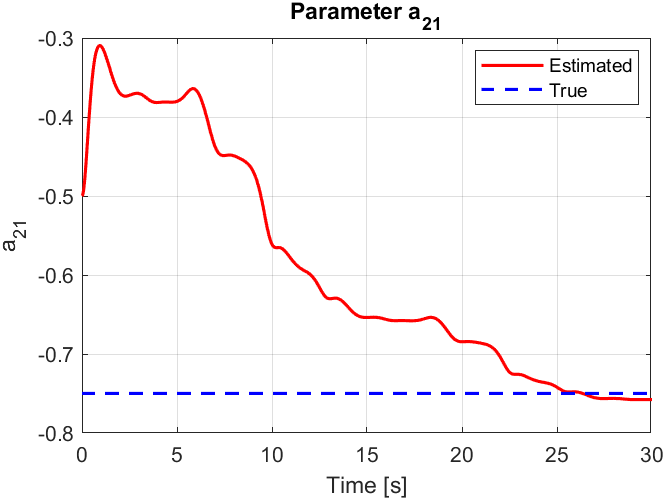
\includegraphics[width=0.8\linewidth]{plots/plot3_c_a21.png}
        % \caption{Image 1}
    \end{minipage}
    \hfill
    \begin{minipage}{0.48\textwidth}
        \centering
        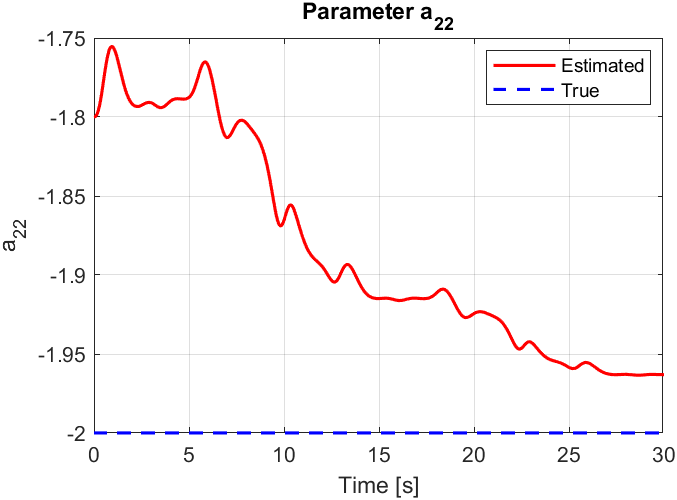
\includegraphics[width=0.8\linewidth]{plots/plot3_d_a22.png}
        % \caption{Image 1}
    \end{minipage}
    
    \caption{}
    \label{fig:A_est}
\end{figure}

\begin{figure}[ht!]
    \centering
    \begin{minipage}{0.48\textwidth}
        \centering
        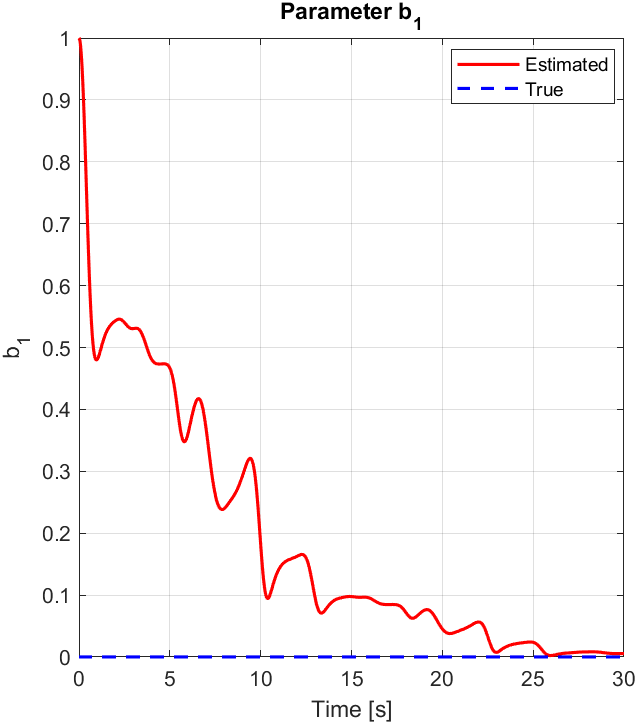
\includegraphics[width=0.7\linewidth]{plots/plot4_a_b1.png}
        % \caption{Image 1}
    \end{minipage}
    \hfill
    \begin{minipage}{0.48\textwidth}
        \centering
        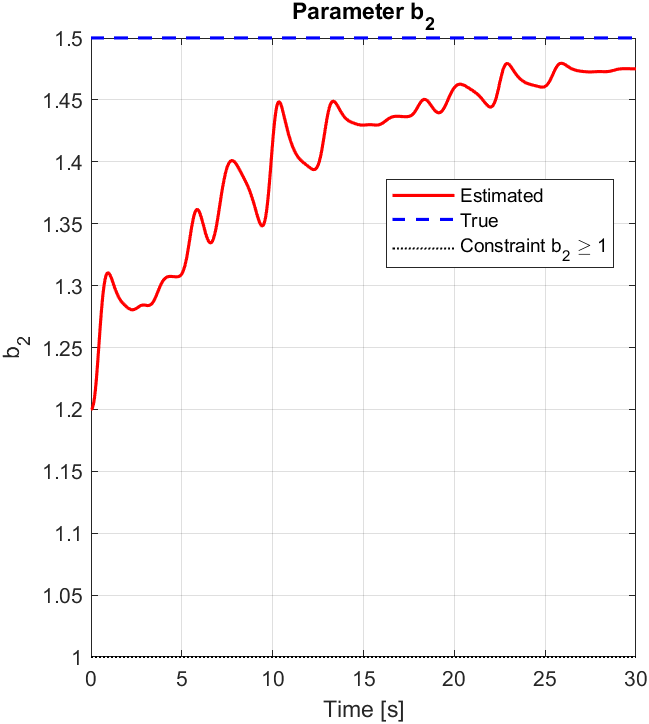
\includegraphics[width=0.7\linewidth]{plots/plot4_b_b2.png}
        % \caption{Image 2}
    \end{minipage}
    
    \vspace{1em} % Space between rows
    
    \centering
    \begin{minipage}{0.48\textwidth}
        \centering
        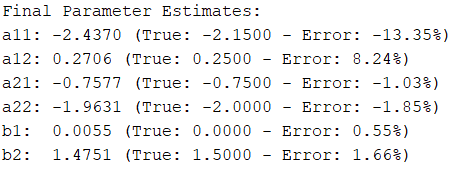
\includegraphics[width=0.8\linewidth]{plots/plot5_logs.png}
        % \caption{Image 1}
    \end{minipage}
    
    \caption{}
    \label{fig:B_est}
\end{figure}



\newpage

\subsection{Ερώτημα Β}

Στην ανάλυση του προβλήματός μας ως τώρα υποθέσαμε την \textit{\textbf{πλήρη γνώση της δομής του συστήματος}} που μελετάμε 
και με βάση αυτήν σχεδιάσαμε έναν τρόπο εκτίμησης των άγνωστων παραμέτρων του (λαμβάνοντας υπόψιν τους δοθέντες περιορισμούς). 
Σε πρακτικές εφαρμογές όμως αυτό είναι ανεφάρμοστο, μιας και πάντα υπάρχουν άγνωστες μη γραμμικότητες που δεν μοντελοποιούνται. 

Γι' αυτόν τον λόγο, σε αυτό το ερώτημα θα εισάγουμε στο σύστημα \textbf{σφάλμα πόλωσης} $\omega \in \mathbb{R}^2$ 
που να ικανοποιεί $||\omega(t)|| \le \bar{\omega}, \forall t \ge 0$, για κάποια άγνωστη σταθερά $\bar{\omega} > 0$.

\subsubsection{Γραμμικά Παραμετροποιημένη Μορφή}

\textit{Πριν το κάνουμε αυτό}, θα φέρουμε το σύστημα \eqref{eq:sys_eq_1} σε γραμμικά παραμετροποιημένη μορφή, ακολουθώντας τα παρακάτω βήματα:

\noindent\textbullet\hspace{0.2em} Αρχικά, ορίζουμε ένα διάνυσμα $\theta^*$ (όπως κάναμε και στο Ερώτημα Α) στο οποίο συγκεντρώνουμε όλες τις προς εκτίμηση παραμέτρους της \eqref{eq:sys_eq_1}:
\vspace{-\topsep}
\vspace{+2pt}
\begin{equation}
   \theta^* = \begin{bmatrix} a_{11} & a_{12} & a_{21} & a_{22} & b_{1} & b_{2} \end{bmatrix}^\top \in \mathbb{R}^6. 
\end{equation}

\noindent Επίσης, ορίζουμε πίνακα $\Delta \in \mathbb{R}^{2 \times 6}$ που περιλαμβάνει όλα τα σήματα εισόδου-εξόδου, ως εξής:
\begin{equation}
\Delta = \begin{bmatrix}
    x_1 & x_2 & 0   & 0   & u & 0 \\
    0   & 0   & x_1 & x_2 & 0 & u
\end{bmatrix}.
\end{equation}

\noindent Σύμφωνα με τα παραπάνω το αρχικό μας σύστημα μπορεί να γραφεί στην μορφή:
\vspace{-\topsep}
\vspace{+2pt}
\begin{equation}\label{eq:sys_linear_param}
    \dot{x} = \Delta \cdot \theta^{*}
\end{equation}

\vspace{-\topsep}
\vspace{+3pt}

\noindent Η παραπάνω μορφή εκφράζει την παράγωγο του διανύσματος $x(t) = \begin{bmatrix} x_1(t) & x_2(t)  \end{bmatrix}^{\top}$ ως το γινόμενο του διανύσματος των παραμέτρων $\theta^{*}$ με τον πίνακα όλων των (γνωστών) σημάτων, $\Delta$.

\vspace{+5pt}

\noindent\textbullet\hspace{0.2em} 
Το σύστημα έχει δύο εξόδους, τις $x_1$ και $x_2$, συνεπώς ορίζουμε $y(t) = x(t)$. 
Για να φέρουμε το σύστημα \eqref{eq:sys_linear_param} στην μορφή $y = \Phi \theta^{*} $\textemdash 
με το $\Phi$ εδώ να είναι πίνακας στο $\mathbb{R}^{2 \times 6}$\textemdash 
πρέπει να απαλλαχθούμε από την παράγωγο $\dot{x}(t)$.
Για να πετύχουμε το ζητούμενο, φιλτράρουμε και τα δύο μέλη της \eqref{eq:sys_linear_param} (κάθε συνιστώσα ξεχωριστά) με κατάλληλης τάξης ευσταθές φίλτρο, $\frac{1}{\Lambda(s)}$.
Για απλότητα και για τις δύο συνιστώσες, μπορούμε να επιλέξουμε ένα φίλτρο πρώτης τάξης, μορφής:
\vspace{-\topsep}
\vspace{+3pt}
\begin{equation}\label{eq:filter}
\frac{1}{\Lambda(s)}, \quad \text{με }\Lambda(s) = s + \lambda,\  \lambda \in \mathbb{R},
\end{equation}
με την ρίζα του πολυωνύμου αυτού να κυμαίνεται στο αριστερό ανοιχτό ημιεπίπεδο, δηλαδή $\lambda > 0$, για να έχουμε ευστάθεια.
Υπενθυμίζουμε ότι και το αρχικό μας σύστημα είναι ευσταθές, μίας και\textemdash όπως αναφέρθηκε και στην εισαγωγική ανάλυση\textemdash 
οι ιδιοτιμές του πίνακα $A$, της \eqref{eq:sys_eq_1}, βρίσκονται στο ανοικτό αριστερό ημιεπίπεδο.


\vspace{+5pt}

\noindent\textbullet\hspace{0.2em} Από την \eqref{eq:sys_linear_param}, παίρνουμε (περνώντας στο πεδίο του Laplace):
\vspace{-\topsep}
\vspace{+3pt}
\begin{equation}\label{eq:sys_param_filter}
  \begin{aligned}
    \left.
      \begin{aligned}
        s X_1 &= a_{11} X_1 + a_{12} X_2 + b_1 U \\
        s X_2 &= a_{21} X_1 + a_{22} X_2 + b_2 U
      \end{aligned}
    \right\}
    &\Rightarrow
    \left.
      \begin{aligned}
        (s + \lambda_1) X_1 &= (a_{11} + \lambda_1) X_1 + a_{12} X_2 + b_1 U \\
        (s + \lambda_2) X_2 &= a_{21} X_1 + (a_{22} + \lambda_2) X_2 + b_2 U
      \end{aligned}
    \right\} \\
    &\Rightarrow
    \left.
      \begin{aligned}
        X_1 &= \frac{a_{11} + \lambda_1}{s + \lambda_1} X_1 + \frac{a_{12}}{s + \lambda_1} X_2 + \frac{b_1}{s + \lambda_1} U \\
        X_2 &= \frac{a_{21}}{s + \lambda_2} X_1 + \frac{a_{22} + \lambda_2}{s + \lambda_2} X_2 + \frac{b_2}{s + \lambda_2} U 
      \end{aligned}
    \right\}
  \end{aligned}
\end{equation}
και όπως βλέπουμε τώρα, καταφέραμε να διώξουμε την παράγωγο και έχουμε απλώς την $x$.

\begin{examplebox}{Σχόλιο}
    Όπως παρατηρούμε, στην \eqref{eq:sys_param_filter} δεν χρειάζεται για κάθε συνιστώσα να έχουμε το ίδιο ακριβώς φίλτρο. 
    Παρόλα αυτά, για απλότητα (και συμμετρία μεταξύ των συνιστωσών) στην ανάλυσης στο MATLAB θα έχουμε $\lambda_1 = \lambda_2 = \lambda$.
\end{examplebox}

Από την \eqref{eq:sys_param_filter} έχουμε ισοδύναμα:
\vspace{-\topsep}
\vspace{+3pt}
\begin{equation}\label{eq:sys_param_filter_2}
\begin{aligned}
        \eqref{eq:sys_param_filter} &\Rightarrow
        \begin{bmatrix}
            X_1 \\ X_2
        \end{bmatrix} = 
        \begin{bmatrix}
            \frac{X_1}{s + \lambda_1}  & \frac{X_2}{s + \lambda_1}  & 0 & 0 & \frac{U}{s + \lambda_1}  & 0 \\ 
            0 & 0 & \frac{X_1}{s + \lambda_2}  & \frac{X_2}{s + \lambda_2}  & 0 & \frac{U}{s + \lambda_2} \\ 
        \end{bmatrix}
        \begin{bmatrix}
            a_{11} + \lambda_1 \\ a_{12} \\ a_{21} \\ a_{22} + \lambda_2 \\ b_1 \\ b_2
        \end{bmatrix} \\
        &\overset{ILT}{\Rightarrow}
        y = \begin{bmatrix}
            x_1 \\ x_2
        \end{bmatrix} = 
        \begin{bmatrix}
            x^{[\lambda_1]}_1  & x^{[\lambda_1]}_2  & 0 & 0 & u^{[\lambda_1]}  & 0 \\ 
            0 & 0 & x^{[\lambda_2]}_1  & x^{[\lambda_2]}_2  & 0 & u^{[\lambda_2]} \\ 
        \end{bmatrix}
        \begin{bmatrix}
            a_{11} + \lambda_1 \\ a_{12} \\ a_{21} \\ a_{22} + \lambda_2 \\ b_1 \\ b_2
        \end{bmatrix}
\end{aligned}
\end{equation}
και επιστρέφοντας στο πεδίο του χρόνου βλέπουμε ότι έχουμε φέρει το σύστημα \eqref{eq:sys_eq_1} σε μορφή $y = \Phi \theta_{\lambda}^{*} $\textemdash 
όπου όλα τα στοιχεία του πίνακα $\Phi \in \mathbb{R}^{2 \times 6}$ είναι γνωστά (μπορούν να υπολογιστούν - αποτελούν τις εξόδους των φίλτρων).

\vspace{+5pt}

\begin{examplebox}{Παρατηρήσεις}
    \begin{enumerate}
        \item Στον τύπο \eqref{eq:sys_param_filter_2}, ο συμβολισμός $x^{[\lambda_j]}_i(t) \in \mathbb{R}, \ i,j \in \{1, 2\},$ χρησιμοποιείται όταν περνάμε με τον αντίστροφο μετασχηματισμό Laplace (ILT) στο πεδίο του χρόνου και αναφέρεται στο σήμα που προκύπτει όταν περάσουμε το αρχικό σήμα $x_i(t)$ από το φίλτρο πρώτης τάξης (της μορφής της \eqref{eq:filter}, για $\lambda = \lambda_j$).

        \item Ο τύπος της \eqref{eq:sys_param_filter_2} μπορεί να γραφεί ξεχωριστά για καθεμία από τις συνιστώσες της $y(t) = \begin{bmatrix}
            y_1(t) & y_2(t)
        \end{bmatrix}^{\top}$ 
        οι οποίες είναι σε γραμμικά παραμετροποιημένη μορφή, μιας και:
        \begin{equation*}
            y_1 = x_1 = 
        \begin{bmatrix}
            x^{[\lambda_1]}_1  & x^{[\lambda_1]}_2  & 0 & 0 & u^{[\lambda_1]}  & 0
        \end{bmatrix}
        \begin{bmatrix}
            a_{11} + \lambda_1 \\ a_{12} \\ a_{21} \\ a_{22} + \lambda_2 \\ b_1 \\ b_2
        \end{bmatrix} = 
        \phi_1 ^{\top} \cdot \theta_{\lambda}^{*} = \theta_{\lambda}^{*\top} \cdot \phi_1 ,
        \end{equation*} 
        και αντίστοιχα για την $y_2(t)$.
    \end{enumerate}
\end{examplebox}

Συνοψίζοντας, φέραμε το σύστημα \eqref{eq:sys_eq_1} στην (γραμμικά παραμετροποιημένη) μορφή $y = \Phi \theta_{\lambda}^{*}$ \eqref{eq:sys_param_filter_2}. 
Σε αυτήν, όπως εξηγήσαμε όλα τα μεγέθη είναι γνωστά και μετρήσιμα/υπολογίσιμα εκτός από το διάνυσμα $\theta_\lambda$\textemdash 
οπότε μπορούμε να προχωρήσουμε την ανάλυσή μας.




\newpage 

\subsubsection{Εισαγωγή Σφάλματος Πόλωσης στο Σύστημα}
Για να καταλήξουμε στην \eqref{eq:sys_param_filter_2} θεωρήσαμε γνωστή, μέσω της \eqref{eq:sys_eq_1}, την δομή του συστήματος που μελετάμε.
Όπως αναφέραμε όμως, σε πρακτικές εφαρμογές πάντα υπάρχουν άγνωστες μη-γραμμικότητες. 
Έτσι, ακόμα και αν γνωρίζαμε το προς εκτίμηση \(\theta^*\), η έξοδος του συστήματος στην πράξη δεν θα περιγράφονταν από την \eqref{eq:sys_param_filter_2} αλλά από την:
\begin{equation}\label{eq:system_polosi}
    y = \Phi \theta_{\lambda}^{*} + \omega, 
\end{equation}
στην οποία, ο όρος \(\omega\) μπορεί να θεωρηθεί ως το σφάλμα προσέγγισης της εξόδου \(y\) του πραγματικού συστήματος από το $\Phi \theta_{\lambda}^{*}$ και στην ανάλυση που κάνουμε για αυτό ισχύει ότι: $||\omega(t)|| \le \bar{\omega}, \forall t \ge 0$, για κάποια άγνωστη σταθερά $\bar{\omega} > 0$.

Για να λύσουμε το πρόβλημα μπορούμε να χρησιμοποιήσουμε την διακοπτική $\sigma$-τροποποίηση η οποία, σύμφωνα με την θεωρία, 
εξασφαλίζει τόσο ότι δεν θα έχουμε παραμετρική ολίσθηση όσο και σύγκλιση του σφάλματος εξόδου στο $0$ (θεωρητικά).
Εφόσον έχουμε ήδη φέρει το σύστημα στην μορφή \eqref{eq:sys_param_filter_2}, στην συνέχεια θα σχεδιάσουμε/εφαρμόσουμε την μέθοδο κλίσης με συνεχή διακοπτική $\sigma$-τροποποίηση για την εύρεση των παραμέτρων $\theta_{\lambda}^{*}$.

Άρα, σύμφωνα με την θεωρία, το σύστημα που χρειάζεται να λύσουμε για την εύρεση των παραμέτρων $\hat\theta_{\lambda}^{*}$, αν δεν είχαμε περιορισμούς για τις επιτρεπτές τιμές αυτών, είναι το εξής:
\begin{align}\label{eq:system_biased_omega}
    y &= \Phi \theta_{\lambda}^{*} + \omega, \quad |\theta_{\lambda}^{*}| \leq M \notag \\
    \hat{y} &= \Phi\hat{\theta}_{\lambda}^{*}  \notag\\
    \dot{\hat{\theta}}_{\lambda}^{*} &= -\sigma_\delta \Gamma \hat{\theta}_{\lambda}^{*} -\Gamma \nabla K(\hat{\theta}_{\lambda}^{*}) \\
    \sigma_\delta &= 
    \begin{cases}
        0, & \text{αν } |\hat{\theta}_{\lambda}^{*}| < M \\
        \sigma \left( \frac{|\hat{\theta}_{\lambda}^{*}|}{M} - 1 \right), & \text{αν } M \leq |\hat{\theta}_{\lambda}^{*}| \leq 2M \\
        \sigma, & \text{αν } |\hat{\theta}_{\lambda}^{*}| > 2M
    \end{cases} \notag,
\end{align}
όπου:
\begin{itemize}[noitemsep, nolistsep]
    \item Το $K(\hat{\theta}_{\lambda}^{*})$ είναι η συνάρτηση κόστους που θέλουμε να ελαχιστοποιήσουμε για $\hat{\theta}_{\lambda}^{*} \in \Theta$. Ως συνάρτηση κόστους επιλέγουμε την $K(\hat{\theta}_{\lambda}^{*}) = \frac{||e||^2}{2} = \frac{||y - \Phi\hat{\theta}_{\lambda}^{*}||^2}{2}$.
    Παραγωγίζοντάς την παίρνουμε $\nabla K(\hat{\theta}_{\lambda}^{*}) = -\Phi^{\top} e$.
    \item Το $M >0$ είναι σταθερά την οποία πρέπει να θέσουμε σε κατάλληλη τιμή\textemdash μέσω trial and error\textemdash για να ικανοποιεί την: $|\theta_{\lambda}^{*}| \leq M$ (άρα πρέπει να οριστεί ίση με έναν αρκούντως μεγάλο θετικό αριθμό). 
    \item Το $\sigma >0$ είναι ο συντελεστής της $\sigma$-τροποποίησης. Θα μπορούσαμε να ορίζουμε διαφορετικό $\sigma$ για κάθε μία εκ των παραμέτρων προς εκτίμηση, $\hat{\theta}_i$, όμως για απλότητα διατηρούμε ίδια τιμή σε όλους. 
\end{itemize}

Για να αξιοποιεί ο αλγόριθμος πραγματικού χρόνου που σχεδιάζουμε την πληροφορία ότι $\hat{\theta}_{\lambda}^{*} \in \,^\lambda\Theta$, 
στην ενημέρωση του $\dot{\hat{\theta}}_{\lambda}^{*}$ που παραθέσαμε στο παραπάνω σύστημα της \eqref{eq:system_biased_omega} 
θα εφαρμόζουμε προβολή στο σύνορο $\,^\lambda\Theta_{b}$ μέσω της σχέσης \eqref{eq:update_theta} (που αναπτύξαμε για τις συνθήκες περιορισμού του προβλήματος). 
Έτσι, μπορούμε να εγγυηθούμε ότι το $\hat{\theta}_{\lambda}^{*}$ δεν θα βγει ποτέ εκτός του συνόλου $\,^\lambda\Theta$.

\noindent\textit{Συμβολισμός}: Το σύνολο $\,^\lambda\Theta$ αποτελεί το σύνολο όλων $\hat{\theta}_{\lambda}^{*}$ που ικανοποιούν τους περιορισμούς για τα $a_{11}$ και $b_2$. Υπάρχει ένα προς ένα αντιστοιχία των στοιχείων του με αυτών του συνόλου $\Theta$.
    

\begin{examplebox}{Παρατήρηση}
    Ο αλγόριθμος που θέλουμε να σχεδιάσουμε είναι πραγματικού χρόνου. 
    Επομένως πρέπει στο σύστημα εξισώσεων της \eqref{eq:system_biased_omega} να συμπεριλάβουμε και τον μηχανισμό με τον οποίο βρίσκουμε τις μη μηδενικές συνιστώσες του πίνακα $\Phi$, για κάθε δεδομένη χρονική στιγμή.
    Από την \eqref{eq:sys_param_filter_2} βλέπουμε ότι για τα μη μηδενικά στοιχεία του πίνακα $\Phi$ 
    (και για $\lambda_1 = \lambda_2 = \lambda$) ισχύει:
    \begin{align*}
        \Phi_{11} &= \frac{X_1}{s + \lambda} \xRightarrow{ILT} \dot\Phi_{11}(t) = x_1(t) - \lambda \Phi_{11}(t), \quad \Phi_{11}(t) = \Phi_{23}(t)\  (\text{για κοινό φίλτρο $\lambda$}), \\
        \Phi_{12} &= \frac{X_2}{s + \lambda} \xRightarrow{ILT} \dot\Phi_{12}(t) = x_2(t) - \lambda \Phi_{12}(t), \quad \Phi_{12}(t) = \Phi_{24}(t)\  (-//-), \\
        \Phi_{15} &= \frac{U}{s + \lambda} \xRightarrow{ILT} \dot\Phi_{15}(t) = u(t) - \lambda \Phi_{15}(t), \quad \Phi_{15}(t) = \Phi_{26}(t)\  (-//-). 
    \end{align*}

    Επομένως, για να έχουμε κάθε χρονική στιγμή την τρέχουσα τιμή του πίνακα $\Phi(t)$, στην επίλυση του συστήματος των διαφορικών με \textit{ode45}
    συμπεριλαμβάνουμε και τις παραπάνω τρεις. 
\end{examplebox}


\subsubsection{Μοντελοποίηση $\omega$ στο MATLAB}
Στην προηγούμενη ενότητα αναφέραμε τον τρόπο με τον οποίο θα εφαρμόσουμε την διακοπτική $\sigma$-τροποποίηση (συνεχής εκδοχή) για την εύρεση των παραμέτρων $\hat\theta^*_\lambda$.
Με αυτήν εξασφαλίζουμε πως δεν θα έχουμε παραμετρική ολίσθηση και ότι το σφάλμα εξόδου, $e = x - \hat x$, θα μπορεί να τείνει στο μηδέν. 
Το μόνο που μένει να μοντελοποιήσουμε ώστε να μπορούμε να περάσουμε το σύστημα της \eqref{eq:system_biased_omega}\footnote{
Όπως το αναλύσαμε στην προηγούμενη ενότητα\textemdash μαζί με τα σχόλια και τις παρατηρήσεις που το συνοδεύουν.
} στο MATLAB είναι το $\omega$.

Το $\omega(t) \in \mathbb{R}^2$ πολώνει την \eqref{eq:sys_param_filter_2} και έτσι μας οδηγήσει στην \eqref{eq:system_polosi}.
Γενικά, το $\omega(t)$ μπορεί να μοντελοποιηθεί ως μικρή διαταραχή χαμηλής συχνότητας. 
Ένας απλός τρόπος μοντελοποίησης θα ήταν να ορίσουμε και τις δύο συνιστώσες ίσες με κάποιο ημίτονο συχνότητας $\omega_{f}$, δηλαδή:
$$
\omega(t) = \begin{bmatrix}
    0.8  \bar\omega \sin(\omega_{f}  t) \\
    0.6  \bar\omega \sin(\omega_{f}  t) 
\end{bmatrix}.
$$
Παρόλο που το παραπάνω αποτελεί έναν απλό τρόπο μοντελοποίησης του $\omega$, θα ισχύει $||\omega|| = \bar\omega, \forall t$.

Για να αποφύγουμε περιπτώσεις σταθερού πλάτους επιλέγουμε για κάθε συνιστώσα να δώσουμε μία διαφορετική μικρή συχνότητα και μια διαφορά φάσης μεταξύ τους. 
Έτσι, στο αρχείο \textit{src/computeBiasError.m} μοντελοποιήσαμε την παρακάτω συνάρτηση για το σφάλμα πόλωσης:
\begin{equation}\label{t1b:omega}
    \omega(t) = \begin{bmatrix}
        0.7  \bar\omega \sin(\omega_{f1}  t) \\
        0.6  \bar\omega \cos(\omega_{f2}  t + \pi/4) 
    \end{bmatrix},
\end{equation}
κάνοντας κατάλληλο έλεγχο έτσι ώστε, αν έχουμε κάποιο πλάτος μεγαλύτερο του $\bar\omega$ να το κάνουμε scale. 

Τα $\omega_{f1}, \omega_{f2}$ ορίζονται στο script \textit{mainTopic1b.m}, στην μεταβλητή {\small\texttt{omega\_freq}}, και είναι ίσα με $0.7$ και $1.2$ αντίστοιχα, για όλες τις περιπτώσεις $\bar\omega$.
Στο αρχείο \textit{normOmega.m} υπολογίζουμε και κάνουμε plot την νόρμα του $\omega$ για να δούμε το πως αυτή κυμαίνεται και αν ικανοποιεί τους περιορισμούς. 

\begin{examplebox}{Σημείωση}
    Από το αρχείο \textit{normOmega.m} είναι φανερό ότι με τον τύπο που δώσαμε για την $\omega(t)$, 
    το $\bar\omega$ αποτελεί το κατώτερο άνω φράγμα για την συνάρτηση της νόρμας $||\omega(t)||$\textemdash
    ακομή και αν δεν κάνουμε έλεγχο για πλάτος μεγαλύτερο του $\bar\omega$ και scale. 
    Επομένως, ο έλεγχος αυτός είναι καθαρά προαιρετικός για την επιλεγμένη μοντελοποίηση που παραθέσαμε. 
\end{examplebox}

\newpage


\subsubsection{Αποτελέσματα MATLAB και Συμπεράσματα}
TODO: \\
- Βάλε πλοτς και πες συμπεράσματα
- πως επηρεάζει το μπαρ-ω την σύγκληση (την κάνει χειρότερη!!)\\



\newpage

\section{Θέμα 2}

Στόχος του θέματος αυτού είναι η μελέτη της \textit{διαδικασίας επιλογής και αξιολόγησης} μοντέλου 
για την προσέγγιση αγνώστου μη-γραμμικού δυναμικού συστήματος της μορφής:
\begin{equation}\label{t2:sys_form}
    \dot x (t) = f(x(t), u(t), \theta), \quad f: \mathbb{R} \times \mathbb{R} \rightarrow \mathbb{R}, 
\end{equation}
με $u(t) \in \mathbb{R}$ και $x(t)\in \mathbb{R}$ να είναι μετρήσιμα και να αποτελούν την είσοδο και την έξοδο του συστήματος, αντίστοιχα, ενώ
$\theta = [\theta_1, \theta_2]^{\top} \in \mathbb{R}^2$ είναι ένα σταθερό διάνυσμα παραμέτρων. 

Για το πραγματικό μη γραμμικό σύστημα που περιγράφεται από την \eqref{t2:sys_form} ισχύει:
\begin{equation}\label{t2:f_true}
    f(x, u, \theta) = - x^3 + \theta_1 \tanh(x) + \theta_2 \frac{1}{1 + x^2} + u, 
\end{equation}
όπου $\theta_1, \theta_2 \in [0.5, 2]$ και $u(t)$ είναι δικής μας επιλογής. 

Σε αυτό το θέμα το δοθέν σύστημα αποτελεί ένα "Μαύρο Κουτί", μιας και στην πράξη δεν έχουμε καμία πληροφορία για την δομή του. 
Αν $S$ είναι το πραγματικό σύστημα, τότε αυτό παίρνει ως είσοδο μια οποιαδήποτε συνάρτηση της επιλογής μας, $u(t)$, 
και δίνει στην έξοδό του την (επίσης μετρήσιμη) συνάρτηση $x(t) = S[u(t)]$.


\subsection{Ερώτημα Α}
Ένα πρώτο βήμα για την κατανόηση του συστήματός μας είναι να ελέγξουμε αν αυτό είναι γραμμικό και χρονοαμετάβλητο.
Για να το κάνουμε αυτό μπορούμε να δοκιμάσουμε να δώσουμε στο σύστημα διάφορα ζεύγη εισόδων $\{u_1(t), u_2(t)\}$
και να ελέγχουμε αν για αυτά ισχύει η σχέση $S[au_1(t) + bu_2(t)] = aS[u_1(t)] + bS[u_2(t)],\ a,b \in \mathbb{R}$.
Αντίστοιχα για τον έλεγχο του αμετάβλητου ως προς το χρόνο μπορούμε να κάνουμε τον έλεγχο για το αν ισχύει η συνεπαγωγή: 
$S[u(t)] = x(t) \Rightarrow S[u(t - t_0)v(t-t_0)] = x(t-t_0)v(t-t_0)$, όπου με $v(t)$ ορίζουμε την βηματική συνάρτηση. 

Τα παραπάνω βέβαια αποτελούν απλώς μία πρώτη επαφή με το σύστημά μας, και μπορούν μόνο να χρησιμοποιηθούν, όχι για να αποδείξουν, αλλά για να 
καταρρίψουν την υπόθεση για γραμμικό ή χρονοαμετάβλητο σύστημα. 

Στην συνέχεια της ανάλυσης θα παρουσιάσουμε την διαδικασία επιλογής δομής που ακολουθήσαμε για την προσέγγιση του αγνώστου συστήματος της \eqref{t2:sys_form}.


\subsubsection{Διαδικασία Επιλογής Δομής}

Ο στόχος εδώ είναι να προσεγγίσουμε την άγνωστη συνάρτηση \(f(x, u, \theta)\) χρησιμοποιώντας μια δομή μοντέλου που συντίθεται από \textit{βασικές συναρτήσεις}. 
Για την διαδικασία επιλογής δομής μοντέλου\textemdash δηλαδή την επιλογή ενός συνόλου βασικών συναρτήσεων \textbf{και} τον προσδιορισμό της πολυπλοκότητάς τους, όπως για παράδειγμα το πλήθος των όρων του\textemdash ακολουθούμε τα παρακάτω βήματα:

1. \textit{Επιλογή Βασικών Συναρτήσεων}: \\
Επιλέγουμε μια "οικογένεια" βασικών συναρτήσεων για να αναπαραστήσουμε τη \(f(x, u, \theta)\). 
Συνήθεις επιλογές περιλαμβάνουν 
πολυώνυμα \( \{1, x, x^2, x^3, \dots, u, u^2, \dots\} \), 
γκαουσιανές βασικές συναρτήσεις (RBFs) \(\phi_i(x) = \exp\left(-\frac{(x - c_i)^2}{2\sigma_i^2}\right)\),
ρητές συναρτήσεις όπως η ίδια η \(\frac{1}{1 + x^2}\), κ.α.


2. \textit{Επιλογή Υποψήφιων Μοντέλων}: \\
Ορίζουμε πολλαπλές δομές μοντέλων με αυξανόμενη πολυπλοκότητα. Οι επιλογές που κάνουμε παρατίθενται παρακάτω:
\begin{itemize}[noitemsep, nolistsep]
    \item Μοντέλο 1 (Απλό Πολυώνυμο): 
    $$\hat{f} = \hat{\theta}_0 + \hat{\theta}_1 x + \hat{\theta}_2 x^2 + \hat{\theta}_3 x^3 + \hat{\theta}_4 u + \hat{\theta}_5 u^2.$$
    
    \item Μοντέλο 2 (Πολυώνυμο + Tanh): 
    $$\hat{f} = \hat{\theta}_0 + \hat{\theta}_1 x + \hat{\theta}_2 x^3 + \hat{\theta}_3 \tanh(x) + \hat{\theta}_4 u.$$
    
    \item Μοντέλο 3 (Γκαουσιανές RBFs): 
    $$\hat{f} = \sum_{i=0}^k \hat{\theta}_i \exp\left(-\frac{(x - c_i)^2}{2\sigma^2}\right) + \hat{\theta}_{k+1} u,\ \text{ με κέντρα \(c_i\) και πλάτος \(\sigma\)}.$$

    \item Μοντέλο 4 (Γκαουσιανές RBFs + Πολυωνυμικός όρος): 
    $$\hat{f} = \hat{\theta}_0 x^3 + \sum_{i=1}^k \hat{\theta}_i \exp\left(-\frac{(x - c_i)^2}{2\sigma^2}\right) + \hat{\theta}_{k+1} u.$$
\end{itemize}

4. \textit{Επιλογές Εισόδου \(u(t)\)}: \\ 
Η είσοδος \(u(t)\) θα πρέπει να επιλεγεί κατάλληλα ώστε να διεγείρει το σύστημα έτσι, ώστε να σκιαγραφείται η δυναμική του. 
Καλές επιλογές που θα χρησιμοποιηθούν στην προσομοίωση είναι αθροίσματα ημιτονοειδών, μιας και με αυτά καλύπτεται ένα εύρος συχνοτήτων. 

5. \textit{Προσομοίωση του Συστήματος}: \\
Τέλος, χρησιμοποιούμε το αληθινό σύστημα \(\dot{x} = -x^3 + \theta_1 \tanh(x) + \theta_2 \frac{1}{1+x^2} + u\) με επιλεγμένα \(\theta_1, \theta_2 \in [0.5, 2]\) (επιλέγουμε για την συνέχεια της ανάλυσής μας \(\theta_1 = 1.5\), \(\theta_2 = 2.0\)) 
για να παράγουμε δεδομένα εξόδου για την προσαρμογή του μοντέλου. 


\subsubsection{Εκτίμηση Παραμέτρων σε Πραγματικό Χρόνο}

Για την εκτίμηση παραμέτρων σε πραγματικό χρόνο, το μοντέλο πρέπει να προσαρμόζει τις παραμέτρους του \(\hat{\theta}\) καθώς νέα δεδομένα \((x(t), u(t))\) γίνονται διαθέσιμα. 
Δεδομένου ότι το σύστημα είναι μη γραμμικό, μπορούμε να χρησιμοποιήσουμε μεθόδους βασισμένες σε κλίση όπως την αναδρομική μορφή της μεθόδου ελαχίστων τετραγώνων (RLS) ή την μέθοδο κλίσης, όπως την παραθέσαμε και στην ανάλυση του προηγούμενου θέματος.

Από την θεωρία έχουμε τα RLS και η μέθοδος κλήσης μπορούν να εφαρμοστούν σε ένα μοντέλο γραμμικό ως προς τις παραμέτρους:
\[
\dot{x}(t) \approx \hat{f}(x, u, \hat{\theta}) = \phi(x, u)^{\top} \hat{\theta} = \hat{\theta}^{\top} \phi(x, u),
\]
όπου \(\phi(x, u) = [\phi_0(x), \dots, \phi_n(x), u]^{\top}\) είναι το διάνυσμα των οπισθοδρομητών και \(\hat{\theta} = [\hat{\theta}_0, \dots, \hat{\theta}_{n+1}]^{\top}\). 

Προφανώς, ακολουθώντας την διαδικασία που αναλύσαμε στο Ερώτημα Β του θέματος 1, μπορούμε μα χρήση κατάλληλου φίλτρου πρώτης τάξης να διώξουμε την παράγωγο $\dot{x}(t)$ και να φέρουμε το σύστημα σε μορφή $y = \theta^{\top} \phi$.

H μέθοδος κλίσης για το πρόβλημά μας δίνει την ανανέωση του $\theta$ σύμφωνα με την:
\[
\dot{\hat{\theta}} = \gamma (y - \hat\theta \phi) \phi = \gamma e \phi,
\]
όπου \(e =  y - \hat\theta \phi\).

Λύνοντας το σύστημα των διαφορικών που προκύπτουν (όπως έχουμε αναφέρει ήδη στο Θέμα 1) θα είμαστε σε θέση να εκτιμήσουμε το διάνυσμα των $\theta$.

\subsubsection{Αξιολόγηση και Σύγκριση Μοντέλων}
Για να συγκρίνουμε τις υποψήφιες δομές μοντέλων, χρειάζεται να αξιολογήσουμε την απόδοσή τους χρησιμοποιώντας ποσοτικές μετρικές και ποιοτική ανάλυση (οπτικοποίηση προβλέψεων).

Μερικές μετρικές αξιολόγησης που μπορούμε να λάβουμε υπόψιν είναι:
\begin{enumerate}[nolistsep, noitemsep]
    \item Μέσο Τετραγωνικό Σφάλμα (MSE) \\
        \[
        \text{MSE} = \frac{1}{T} \int_0^T (\dot{x}(t) - \hat{f}(x(t), u(t), \hat{\theta}(t)))^2 \, dt,
        \]
        προσεγγιζόμενο διακριτά σε χρονικά βήματα. Χαμηλότερο MSE δείχνει καλύτερη προσαρμογή.
    
    \item Κριτήριο Πληροφορίας Akaike (AIC) \\
        \[
        \text{AIC} = 2k + N \ln(\text{MSE}),
        \]
        όπου \(k\) είναι ο αριθμός των παραμέτρων, και \(N\) είναι ο αριθμός των σημείων δεδομένων. Το AIC εξισορροπεί την προσαρμογή του μοντέλου (MSE) και την πολυπλοκότητα (αριθμός παραμέτρων).
        
    \item Εγκάρσια Αξιολόγηση (Cross Validation - CV) \\
       - Χωρίστε τα δεδομένα σε σύνολα εκπαίδευσης και επικύρωσης (π.χ., 70% εκπαίδευση, 30% επικύρωση).
   - Προσαρμόστε το μοντέλο στο σύνολο εκπαίδευσης και υπολογίστε MSE στο σύνολο επικύρωσης για να αξιολογήσετε τη γενίκευση.
\end{enumerate}



\newpage

\end{document}
